
\begin{table}[!t]
\centering
    \caption{Summary of the data distribution}
    \label{tab:data}
    \rowcolors{2}{white}{gray!10}
\begin{tabular}{r|rrrr}
\toprule
Project & \# train & \# labels & imbalance\% & \# test \\
\midrule
 maven & 2 & 1 & 33 & 1 \\
 cassandra & 9 & 4 & 38 & 4 \\
 jmeter & 10 & 4 & 43 & 4 \\
 commons & 12 & 5 & 59 & 5 \\
 lucene-solr & 19 & 5 & 38 & 6 \\
 ant & 22 & 6 & 36 & 7 \\
 tomcat & 134 & 13 & 41 & 37 \\
 derby & 346 & 20 & 37 & 92 \\
 \midrule
 total & 554 & 58 & & 156 \\
 \bottomrule
\end{tabular}
\end{table}
\begin{table*} 
    \centering
    \caption{Design of our ablation study. 
    %In the header, \textbf{B} = boundary engineering, \textbf{Le} = label engineering, \textbf{Lc} = learner choice, \textbf{H} = hyper-parameter engineering, \textbf{I} = instance engineering. 
    In the learner choice column, \textbf{F} = feedforward networks, \textbf{T} = traditional learners, \textbf{C} = CNN, \textbf{B} = CodeBERT. 
    }
    \label{tab:treatments}
    \footnotesize
    \rowcolors{2}{white}{gray!10}
    \adjustbox{max width=\linewidth}{
    \begin{tabularx}{\linewidth}{r|lllll|rL}
        \toprule
        & \multicolumn{5}{c|}{Engineering decisions}&\\\cline{2-6}
        Treatment & \begin{turn}{70} Boundary    \end{turn} & \begin{turn}{70} Label   \end{turn} & \begin{turn}{70} Learner  \end{turn} & \begin{turn}{70}  Parameter   \end{turn} & \begin{turn}{70} Instance    \end{turn} & \% Labels  & Description \\
        \midrule
        A1   & \tick & \tick & F & \tick & \tick & 10 & Our recommended method \\
        A2 & \tick & \tick & F & \tick & & 10 & A1 without instance engineering (no SMOTE) \\
        A3 & \tick & \tick & F & & \tick & 10 & A1 without hyper-parameter engineering (no DODGE) \\
        A4 & & \tick & F & \tick & \tick & 10 & A1 without boundary engineering (no GHOST) \\
        A5 & \tick & & F & \tick & \tick & 100 & A1 without label engineering (no SMOOTH). From TSE'21~\cite{yedida2021value} \\
        A6 & \tick & & T & \tick & \tick & 100 & A1 without label engineering, replacing feedforward with traditional learners \\
        A7 & \tick & \tick & T & \tick & \tick & 10 & A1 replacing feedforward with traditional  learners \\
        B1 & & \tick & T & \tick & \tick & 10 & A1 without boundary engineering, replacing feedforward with traditional learners \\
        B2 & & \tick & C & \tick & \tick & 10 & A1 without boundary engineering, replacing feedforward with CNN \\
        C1 & & & T & \tick & \tick & 100 & A1 without boundary engineering or label engineering, replacing feedforward with traditional learners \\
        C2 & & & C & \tick & \tick & 100 & A1 without boundary engineering or label engineering, replacing feedforward with CNN \\
        D1 & & & T & & \tick & 100 & Setup used by the \citet{yang2021learning} and \citet{kang2022detecting} studies. \\
        CodeBERT & & & B & & & 100 & CodeBERT without modifications \\\bottomrule
    \end{tabularx} }
\end{table*}
\subsection{Experimental Rig}\label{rigg}
 This study explores:
 \bi
 \item
   $N=4$ pre-processors 
 (boundary, label, parameter, instance)
 that could be mixed in $2^4=16$ ways.
 \item
 Six  traditional learners:  logistic regression, decision trees,
 random forests,
 SVMs (with 3  basis functions);
 \item 
 Three neural net architectures: CNN, CodeBERT, feedforward networks;
 \ei
  To clarify  the reporting of these $16\times(6+3) = 144$ treatments, we made the following decisions.
  Firstly, 
  when reporting the results of the traditional learner, just show the results of the one that beat the other traditional learners   (which, in our case, was typically random forest or logistic regression).
 
Secondly, we 
  do not apply pre-processing or parameter engineering
  on CodeBERT. This decision was required, for pragmatic reasons. Due to  the computational cost of training
  that model,  we could  only  run   off-the-shelf CodeBERT.
 
 Thirdly, 
  rather than explore all 16 combinations of use/avoid
  different pre-processing, we  ran the {\em ablation study}
  recommended in Cohen's
  {\em Empirical
     Methods for AI} textbook~\cite{cohen1995empirical}.
    Ablation studies let us explore some combination of
     $N$ parts can be assessed in time $O(N)$, not $O(2^N)$.
     Such   ablation studies work as follows:
     \bi
     \item Commit to a preferred approach, with $N$ parts;
     \item If removing any  part $n_i\in N$ degrades performance, then conclude that  all  $N$ parts are useful.
     \ei
 With these decisions, 
 instead of having to report on 144 treatments,
 we need only show the 13 treatments in the  ablation study of
Table~\ref{tab:treatments}.
% In that table:
% \bi
% \item
% The treatment A1 applies    all our pre-processors to the training data. 
% \item
% Treatments A2,A3,A4 A5,A6,A7 delete different parts of the A1 assembly;
% \item
% Treatments B1,B2 ignores boundary engineering and tries different internal learners;
% \item
% Treatmetns C1,C2 ignores boundary engineering {\em and} label engineering (with  different internal learners);
% \item 
% Treatments D1 reproduces prior results from 
%  \citet{yang2021learning} and \citet{kang2022detecting};
%  \item
%  Treatment CodeBERT tries a state-of-the-art method (a neural net trained on millions of samples from contemporary SE projects~\cite{feng2020codebert}); 
% \ei
In that table,
for treatments that use any of boundary  
or label or parameter or instance engineering,
we apply those treatments in the  order  recommended by  the original  GHOST paper~\cite{yedida2021value}. That paper
 found  that it could improve  recall by 30\% (or more) by multiple rounds of SMOTE + GHOST. As per that advice,
 A1  executes our pre-processors in the  order:
   \[ \mathit{smote} \rightarrow  \mathit{ghost} \rightarrow \mathit{ghost} \rightarrow \mathit{smote} \rightarrow \mathit{smooth} \rightarrow  \mathit{dodge}\]
  
This paper does not explore the effect of different orderings; rather, our core idea is that the different engineering techniques work together to produce strong results. We leave the exploration of the effect of ordering to future work. 
  
All the treatments labelled ``A'' (A1,A2,A3,A4,A5)  in Table~\ref{tab:treatments},  use the order shown above, perhaps
(as part of the ablation study) skipping over one or more the steps. 
We acknowledge that there are many possible ways to order the applications of our treatments, which is a matter we will for future work. For the moment,the ordering shown above seems useful (evidence: see next section).


% \begin{figure*}[!t] 
%     \centering
%     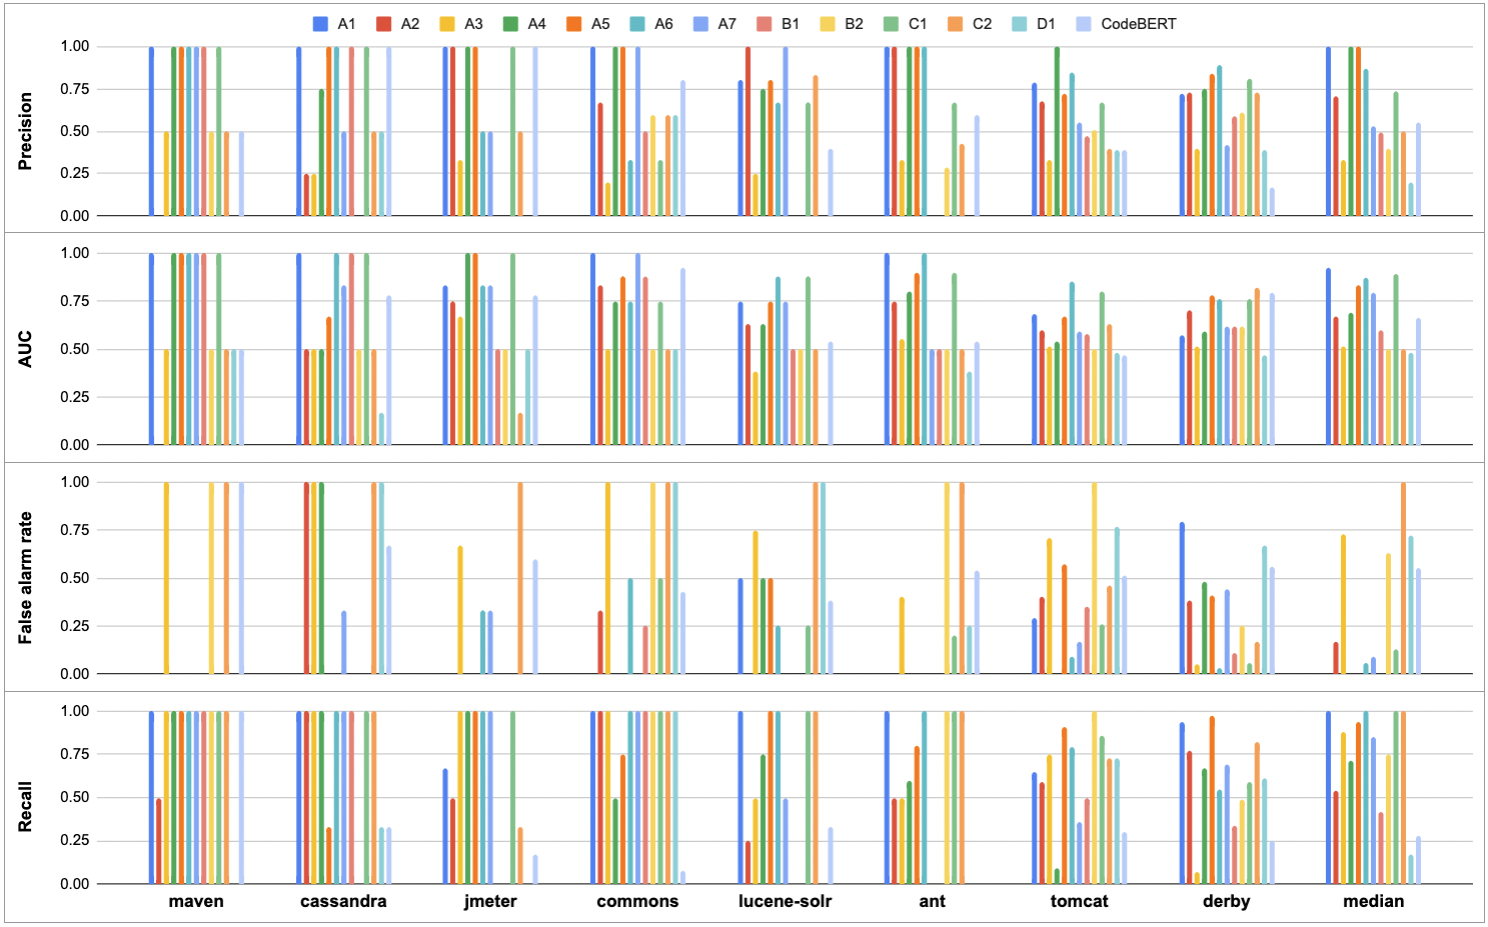
\includegraphics[width=\linewidth]{rahul/results.png}
%     \caption{Results of the ablation study (and for a  partial summary of these results, see Table~\ref{summary}).
%     The treatments A1,A2,A3,A4,A5,A6,A7,B1,B2,C1,C2,D1,Codebert are defined in Table~\ref{tab:treatments}.
%     Each treatment is
%     assessed using the metrics defined in
%     Table~\ref{tab:metrics}. Data sets are ordered left to right, smallest to largest (for details, see Table~\ref{tab:data}).
%       Median results shown on the right-hand-side.  }
%     \label{fig:results}
% \end{figure*}

\newcommand{\best}{\cellcolor{lightgray}}
\newcommand{\bad}{\cellcolor{pink}}

\begin{table*}[t]
\renewcommand{\baselinestretch}{.5}
{ 
   
    \caption{Our results across eight datasets on four metrics.}
    \label{tab:results}
   \scriptsize

    \begin{center}
    \begin{tabular}{l|llllllll|l}
    
        \toprule   
        \textbf{Treatment} & \textbf{maven} & \textbf{cassandra} & \textbf{jmeter} & \textbf{commons} & \textbf{lucene-solr} & \textbf{ant} & \textbf{tomcat} & \textbf{derby} & \textbf{median} \\
        \midrule
        \multicolumn{10}{c}{PRECISION  ({\em better} results are {\em larger})} \\
        \midrule
A1                      & 1   & 1    & 1    & 1    & 0.8  & 1    & 0.79 & 0.72 & 1             \\
A2                      & \bad 0   & \bad 0.25 & 1    & \bad 0.67 & 1    & 1    & \bad 0.68 & 0.73 & \bad 0.71          \\
A3                      & \bad 0.5 & \bad 0.25 & \bad 0.33 & \bad 0.2  & \bad 0.25 & \bad 0.33 & \bad 0.33 & \bad 0.4  & \bad 0.33          \\
A4                      & 1   & 0.75 & 1    & 1    & 0.75 & 1    & 1    & 0.75 & 1             \\
A5                      & 1   & 1    & 1    & 1    & 0.8  & 1    & 0.72 & 0.84 & 1             \\
A6                      & 1   & 1    & \bad 0.5  & \bad 0.33 & \bad 0.67 & 1    & 0.85 & 0.89 & 0.87 \\
A7                      & 1   & \bad 0.5  & \bad 0.5  & 1    & 1    & \bad 0    & \bad 0.55 & \bad 0.42 & \bad 0.53          \\
B1 (DODGE)              & 1   & 1    & \bad 0    & \bad 0.5  & \bad 0    & \bad 0    & \bad 0.47 & \bad 0.59 & \bad 0.49          \\
B2 (CNN)                & \bad 0.5 & \bad 0    & \bad 0    & \bad 0.6  & \bad 0    & \bad 0.29 & \bad 0.51 & \bad 0.61 & \bad 0.4           \\
C1 (DODGE)              & 1   & 1    & 1    & \bad 0.33 & \bad 0.67 & \bad 0.67 & \bad 0.67 & 0.81 & \bad 0.74          \\
C2 (CNN)                & \bad 0.5 & \bad 0.5  & \bad 0.5  & \bad 0.6  & 0.83 & \bad 0.43 & \bad 0.4  & 0.73 & \bad 0.5           \\
D1                      & \bad 0   & \bad 0.5  & \bad 0    & \bad 0.6  & \bad 0    & \bad 0    & \bad 0.39 & \bad 0.39 & \bad 0.2           \\
CodeBERT & \bad 0.5 & 1    & \bad 0.8    & \bad 0.63  & \bad 0.6  & \bad 0  & \bad 0.41 & \bad 0.25 & \bad 0.55 \\
    \midrule 
    \multicolumn{10}{c}{AUC: TP vs. TN ({\em better} results are {\em larger})}   \\
    \midrule
A1                   & 1   & 1    & 0.83 & 1    & 0.75 & 1    & 0.68 & 0.57 & 0.92          \\
A2                   & \bad 0   & \bad 0.5  & 0.75 & 0.83 & 0.63 & 0.75 & 0.6  & 0.7  & \bad 0.67          \\
A3                   & \bad 0.5 & \bad 0.5  & \bad 0.67 & \bad 0.5  & \bad 0.38 & \bad 0.55 & \bad 0.51 & 0.51 & \bad 0.51          \\
A4                   & 1   & 0.5  & 1    & 0.75 & 0.63 & 0.8  & 0.54 & 0.59 & 0.69          \\
A5                   & 1   & 0.67 & 1    & 0.88 & 0.75 & 0.9  & 0.67 & 0.78 & 0.83          \\
A6                   & 1   & 1    & 0.83 & 0.75 & 0.88 & 1    & 0.85 & 0.76 & 0.87 \\
A7                   & 1   & 0.83 & 0.83 & 1    & 0.75 & 0.5  & 0.59 & 0.62 & 0.79          \\
B1 (DODGE)           & 1   & 1    & 0.5  & 0.88 & 0.5  & 0.5  & 0.58 & 0.62 & 0.6           \\
B2 (CNN)             & \bad 0.5 & \bad 0.5  & \bad 0.5  & \bad 0.5  & \bad 0.5  & \bad 0.5  & \bad 0.5  & 0.62 & \bad 0.5           \\
C1 (DODGE)           & 1   & 1    & 1    & 0.75 & 0.88 & 0.9  & 0.8  & 0.76 & 0.89          \\
C2 (CNN)             & \bad 0.5 & \bad 0.5  & \bad 0.17 & \bad 0.5  & \bad 0.5  & \bad 0.5  & 0.63 & 0.82 & \bad 0.5           \\
D1                   & \bad 0.5 & \bad 0.17 & \bad 0.5  & \bad 0.5  & \bad 0    & \bad 0.38 & \bad 0.48 & \bad 0.47 & \bad 0.48          \\
CodeBERT & \bad 0.5 & \bad 0.56 & \bad 0.68 & \bad 0.53 & \bad 0.63 & \bad 0.48 & \bad 0.44 & 0.63 & \bad 0.54 \\
    \midrule
    \multicolumn{10}{c}{FALSE ALARM RATE ({\em better} results are {\em smaller})} \\
    \midrule
A1                     & 0 & 0    & 0    & 0    & 0.5  & 0    & 0.29 & 0.79 & 0             \\
A2                     & 0 & 1    & 0    & 0.33 & 0    & 0    & 0.4  & 0.38 & 0.17          \\
A3                     & \bad 1 & \bad 1    & \bad 0.67 & \bad 1    & \bad 0.75 & \bad 0.4  & \bad 0.71 & 0.05 & \bad 0.73          \\
A4                     & 0 & 1    & 0    & 0    & 0.5  & 0    & 0    & 0.48 & 0             \\
A5                     & 0 & 0    & 0    & 0    & 0.5  & 0    & 0.57 & 0.41 & 0             \\
A6                     & 0 & 0    & 0.33 & 0.5  & 0.25 & 0    & 0.09 & 0.03 & 0.06 \\
A7                     & 0 & 0.33 & 0.33 & 0    & 0    & 0    & 0.17 & 0.44 & 0.09          \\
B1 (DODGE)             & 0 & 0    & 0    & 0.25 & 0    & 0    & 0.35 & 0.11 & 0             \\
B2 (CNN)               & \bad 1 & 0    & 0    & \bad 1    & 0    & \bad 1    & \bad 1    & 0.25 & \bad 0.63          \\
C1 (DODGE)             & 0 & 0    & 0    & 0.5  & 0.25 & 0.2  & 0.26 & 0.06 & 0.13          \\
C2 (CNN)               & \bad 1 & \bad 1    & \bad 1    & \bad 1    & \bad 1    & \bad 1    & 0.46 & 0.17 & \bad 1             \\
D1                     & 0 & \bad 1    & 0    & \bad 1    & \bad 1    & \bad 0.25 & \bad 0.77 & \bad 0.67 & \bad 0.72          \\
CodeBERT & \bad 1 & 0 & \bad 0.2  & \bad 1 & 0.25 & \bad 0 &  0.28 &  0.17 & \bad 0.23\\
    \midrule
    \multicolumn{10}{c}{RECALL  ({\em better} results are {\em larger})} \\
    \midrule
A1                     & 1   & 1    & 0.67 & 1    & 1    & 1   & 0.65 & 0.94 & 1 \\
A2                     & \bad 0.5 & 1    & \bad 0.5  & 1    & \bad 0.25 & \bad 0.5 & 0.59 & \bad 0.77 & \bad 0.54       \\
A3                     & 1   & 1    & 1    & 1    & 0.5  & 0.5 & 0.75 & 0.07 & 0.88       \\
A4                     & 1   & 1    & 1    & \bad 0.5  & \bad 0.75 & \bad 0.6 & \bad 0.09 & \bad 0.67 & \bad 0.71       \\
A5                     & 1   & \bad 0.33 & 1    & \bad 0.75 & 1    & \bad 0.8 & 0.91 & 0.97 & 0.94       \\
A6                     & 1   & 1    & 1    & 1    & 1    & 1   & 0.79 & 0.55 & 1 \\
A7                     & 1   & 1    & 1    & 1    & 0.5  & 0   & 0.36 & 0.69 & 0.85       \\
B1 (DODGE)             & 1   & 1    & \bad 0    & 1    & \bad 0    & \bad 0   & \bad 0.5  & \bad 0.34 & \bad 0.42       \\
B2 (CNN)               & 1   & 0    & 0    & 1    & 0    & 1   & 1    & 0.49 & 0.75       \\
C1 (DODGE)             & 1   & 1    & 1    & 1    & 1    & 1   & 0.86 & 0.59 & 1          \\
C2 (CNN)               & 1   & 1    & 0.33 & 1    & 1    & 1   & 0.73 & 0.82 & 1 \\
D1                     & \bad 0   & \bad 0.33 & \bad 0    & 1    & \bad 0    & \bad 0   & \bad 0.73 & \bad 0.61 & \bad 0.17       \\
CodeBERT & 1   & \bad 0.33 & 0.67 &  1 & \bad 0.5 & \bad 0   & \bad 0.26  & \bad 0.25 &  \bad 0.42 \\
    \bottomrule
    \end{tabular}
    \end{center}
}
\end{table*}
 


As to the specifics of the other treatments:
\bi
\item
Treatment A5 is the treatments from the TSE'21 paper  that   proposed GHOSTing~\cite{yedida2021value}.
\item Treatment D1 contains the treatments applied in prior papers by   Yang et al.~\cite{yang2021learning}  and Kang et al. ~\cite{kang2022detecting}.
\item Anytime we applied {\em parameter engineering},
this meant that some automatic algorithm (DODGE) selected the control parameters for the learners (otherwise, we just used the default off-the-shelf settings). 
\item Anytime we apply {\em label engineering}, we are only
used 10\% of the labels in the training data.
\item The last line, showing CodeBERT, has no pre-processing or tuning. As said   above, CodeBERT is so complex that we must  run it ``off-the-shelf''.
\ei

 
% We now discuss our updated approach, which we recommend. We start by combining the train and test set data. We split this data 80/20 into train and test sets (exception: for maven, we split 50/50, since there are only 4 samples in total). We discard all non-numeric columns. We set the ``closed'' label to 1 and the ``open'' label to 0. This is because in doing this, the class imbalance ratio is below 0.5, which is in agreement with the original domain of GHOST (defect prediction). Indeed, by setting the labels to the reverse, our results were worse. This is not by coincidence: because we followed the GHOST algorithm from \citet{yedida2021value}, we also ended up using their weighted loss function. Such a loss function is inherently asymmetric, making the two learning problems (with each set of labels) different, one more difficult than the other.


% At this point, we use SMOTE (i.e., instance engineering), followed by two rounds of fuzzy sampling (boundary engineering) and then SMOTE again. Note that the process of using two rounds of fuzzy sampling followed by SMOTE was recommended by the original GHOST paper Finally, we use DODGE to optimize the number of layers and the number of units per layer in a feedforward network. In essence, our approach is GHOST with the addition of label engineering (and the additional SMOTE step).

% \subsection{Fuzzy sampling and $\beta-$smoothness}

% \begin{figure*}[t]
%     \centering
%     \begin{subfigure}{.49\linewidth}
%         \centering
%         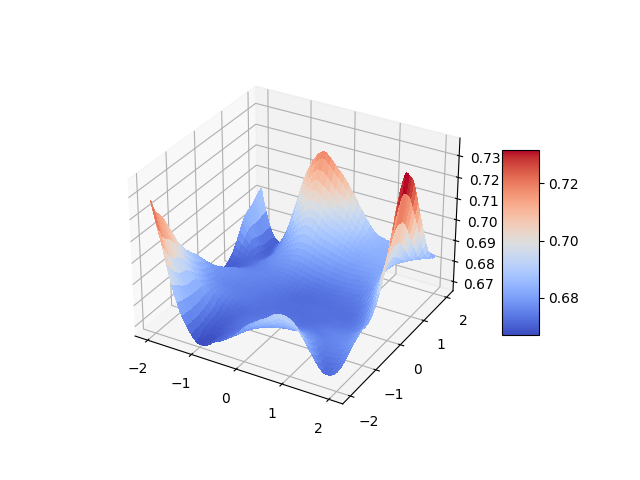
\includegraphics[width=\textwidth]{rahul/tomcat-pre.png}
%         \caption{Before fuzzy sampling}
%     \end{subfigure}
%     \begin{subfigure}{.49\linewidth}
%         \centering
%         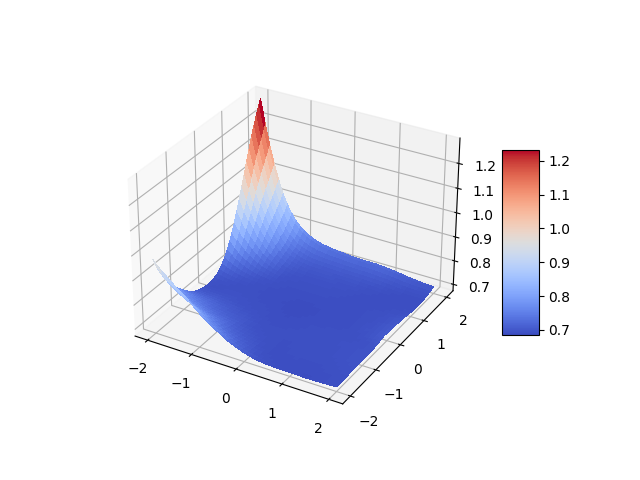
\includegraphics[width=\textwidth]{rahul/tomcat-post.png}
%         \caption{After fuzzy sampling}
%     \end{subfigure}
%     \caption{Loss landscape surface (a) before and (b) after fuzzy sampling.}
%     \label{fig:loss}
% \end{figure*}

% We prove here that fuzzy sampling improves the smoothness of the loss function, making optimization easier. We begin by using the approach of \citet{li2018visualizing} to visualize the loss landscapes before and after using fuzzy sampling. Figure \ref{fig:loss} shows the results of this on the tomcat dataset. Notice that after using fuzzy sampling, the loss surface is significantly smoother. We notice this pattern continue across all our datasets.

% Next, we formalize this notion of smoothness. Recall that the $\beta-$smoothness is defined as the maximum value of $\beta$ for which $\lVert \nabla f(x_1) - \nabla f(x_2) \rVert \leq \beta \lVert x_1 - x_2 \rVert$ under some norm (we use the $l_2$ norm), and is a measure of the smoothness of the loss surface (i.e., higher the $\beta-$smoothness, smoother the loss surface). This is merely the gradient of the Lipschitz constant, which for the binary cross-entropy loss, \citet{yedida2021lipschitzlr} derived as

% \[
%     \frac{\partial^2 \mathcal{L}}{\partial w^{[L]2}_{ij}} = \frac{1}{m} g(\boldsymbol z^{[L]}) (1 - g(\boldsymbol z^{[L]})) a^{[L-1]}_j
% \]

% (here, $\mathcal{L}$ is the loss function, $\boldsymbol w^{[L]}$ is the weight matrix at layer $L$, $L$ is the number of layers, $m$ is the number of training examples in a batch, $g$ is the activation function (at layer $L$, this is the sigmoid function), $\boldsymbol a^{[L-1]}$ is the activation vector at layer $L-1$, and $\boldsymbol z^{[L]}$ is the pre-activation vector, $\boldsymbol z^{[L]} = \boldsymbol W^{[L]T} a^{[L-1]} + b^{[L]}$ for bias vector $b^{[L]}$)

% \begin{table}[h]
%     \centering
%     \caption{Percent changes in the $\beta-$smoothness after fuzzy sampling.}
%     \label{tab:fuzzy}
%     \begin{tabular}{ll}
%         \toprule
%         \textbf{Dataset} & \textbf{\% change} \\
%         \midrule
%         ant & 24.78 \\
%         cassandra & 73.09 \\
%         commons & 29.61 \\
%         derby & 31.35 \\
%         jmeter & 55.53 \\
%         lucene-solr & 16.46 \\
%         maven & 158.87 \\
%         tomcat & 36.34 \\
%         \midrule
%         \textbf{median} & \textbf{33.85} \\
%         \bottomrule
%     \end{tabular}
% \end{table}

% $a^{[L-1]}_j$ is a constant with respect to $\boldsymbol w^{[L]}_{ij}$; for the others, it is trivial to show that an extremum occurs at $\boldsymbol z^{[L]} = 0$, so that $g(\boldsymbol z^{[L]}) = \frac{1}{2}$. Therefore, the $\beta-$smoothness is

% \[
%     \beta = \frac{1}{4m} \max\limits_j \Vert a_j^{[L-1]} \rVert
% \]  

% Because the numerator needs to be computed experimentally, we use this equation to compute the $\beta-$smoothness of the loss surface for each dataset before and after fuzzy sampling. Table \ref{tab:fuzzy} shows the percent changes of the $\beta-$smoothness after using fuzzy sampling. For all datasets, this percent change is positive and significant. Finally, we note that the $\beta-$smoothness is independent of the labels, so the gains from label engineering are independent of the gains from fuzzy sampling.
